
% https://www.writelatex.com/coursera/latex/5.1

\documentclass[t]{beamer}  % [t], [c], или [b] --- вертикальное выравнивание на слайдах (верх, центр, низ)
%\documentclass[handout]{beamer} % Раздаточный материал (на слайдах всё сразу)
%\documentclass[aspectratio=169]{beamer} % Соотношение сторон

%\usetheme{Berkeley} % Тема оформления
%\usetheme{Bergen}
%\usetheme{Szeged}

%\usecolortheme{beaver} % Цветовая схема
%\useinnertheme{circles}
%\useinnertheme{rectangles}


%%% Работа с русским языком
\usepackage{cmap}					% поиск в PDF
\usepackage{mathtext} 				% русские буквы в формулах
\usepackage[T2A]{fontenc}			% кодировка
\usepackage[utf8]{inputenc}			% кодировка исходного текста
\usepackage[english,russian]{babel}	% локализация и переносы

%% Beamer по-русски
\newtheorem{rtheorem}{Теорема}
\newtheorem{rproof}{Доказательство}
\newtheorem{rexample}{Пример}
\newtheorem{rstate}{Утверждение}

%%% Дополнительная работа с математикой
\usepackage{amsmath,amsfonts,amssymb,amsthm,mathtools} % AMS
\usepackage{icomma} % "Умная" запятая: $0,2$ --- число, $0, 2$ --- перечисление

%% Номера формул
%\mathtoolsset{showonlyrefs=true} % Показывать номера только у тех формул, на которые есть \eqref{} в тексте.
%\usepackage{leqno} % Нумерация формул слева

\usepackage{animate}
\usepackage[english]{babel}
%% Перенос знаков в формулах (по Львовскому)
\newcommand*{\hm}[1]{#1\nobreak\discretionary{}
	{\hbox{$\mathsurround=0pt #1$}}{}}

%%% Работа с картинками
\usepackage{graphicx}  % Для вставки рисунков
\graphicspath{{images/}{images2/}}  % папки с картинками
\setlength\fboxsep{3pt} % Отступ рамки \fbox{} от рисунка
\setlength\fboxrule{1pt} % Толщина линий рамки \fbox{}
\usepackage{wrapfig} % Обтекание рисунков текстом

%%% Работа с таблицами
\usepackage{array,tabularx,tabulary,booktabs} % Дополнительная работа с таблицами
\usepackage{longtable}  % Длинные таблицы
\usepackage{multirow} % Слияние строк в таблице


\usepackage{color} %% это для отображения цвета в коде
\usepackage{listings} %% собственно, это и есть пакет listings

\usepackage{caption}
\DeclareCaptionFont{white}{\color{white}} %% это сделает текст заголовка белым
%% код ниже нарисует серую рамочку вокруг заголовка кода.
\DeclareCaptionFormat{listing}{\colorbox{gray}{\parbox{\textwidth}{#1#2#3}}}
\captionsetup[lstlisting]{format=listing,labelfont=white,textfont=white}

%%% Программирование
\usepackage{etoolbox} % логические операторы

%%% Другие пакеты
\usepackage{lastpage} % Узнать, сколько всего страниц в документе.
\usepackage{soul} % Модификаторы начертания
\usepackage{csquotes} % Еще инструменты для ссылок
%\usepackage[style=authoryear,maxcitenames=2,backend=biber,sorting=nty]{biblatex}
\usepackage{multicol} % Несколько колонок
\usepackage[utf8]{inputenc}
%%% Картинки
\usepackage{tikz} % Работа с графикой
\usepackage{pgfplots}
\usepackage{pgfplotstable}

\title{Сортировки за линейное время}
%\author{Данил Фёдоровых}

%\institute[Высшая школа экономики]{Национальный исследовательский университет \\ <<Высшая школа экономики>>}

\begin{document}
	
	\frame[plain]{\titlepage}	% Титульный слайд
	
	
\begin{frame}[t]
	\frametitle{Понятие сортировки}
		\begin{itemize}
	\item \textbf{Cортировкa} — это алгоритм для упорядочивания элементов в списке. \pause
		\item \textbf{Время работы}. Минимальное время работы алгоритма на каком-либо наборе. \pause
		\item  \textbf{Память}. 
		Параметр сортировки, показывающий, сколько дополнительной памяти требуется алгоритму.
        \pause
        \item  \textbf{Устойчивость}. 
        Устойчивой сортировкой называется сортировка, не меняющая порядка объектов с одинаковыми значениями.
		\end{itemize}
\end{frame}

\begin{frame}[t]
	\frametitle{Понятие сложности алгоритма}
		\begin{itemize}
			\pause
        	\item	Под сложностью алгоритма понимается зависимость объёма работы, от размера входных данных.\pause
        	\item фраза «сложность алгоритма есть O(f(n))» означает, что с увеличением параметра n, характеризующего количество входной информации алгоритма, время работы алгоритма будет возрастать не быстрее, чем некоторая константа, умноженная на f(n).\pause
        	\item O() исключает коэффициенты и члены меньшего порядка.\pause
        	\item Говорят, что алгоритм работает за линейное время, или O(n), если его сложность равна O(n). Неформально, это означает, что для достаточно большого размера входных данных время работы увеличивается линейно от размера входа. 
    	\end{itemize}
\end{frame}

\begin{frame}[t]
	\frametitle{Понятие сложности алгоритма}

	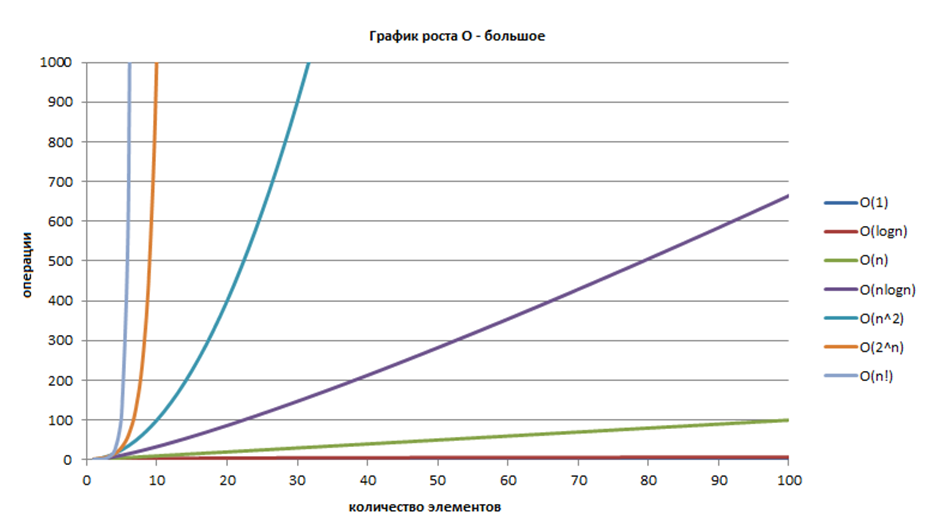
\includegraphics[width=330px,height=220px]{graph1.png}

\end{frame}

\begin{frame}[t]
	\frametitle{Мотивация}
		\begin{itemize}
			\pause
	\item Ускорение обработки данных. \pause
	\item Упрощение обработки данных.  \pause
	\item Зачем столько разных алгоритмов сортировки?  \pause
\end{itemize}
\end{frame}

\begin{frame}[t]
	\frametitle{Counting Sort}
	\begin{itemize}
		\pause
		\item Идея алгоритма заключается в следующем: сначала создается вспомогательный массив, равный длине исходного массива, поданного на сортировку. Последовательно для всех элементов исходного массива выполняется проход, цель которого определить, сколько раз каждый элемент встречается в исходном массиве. Эти данные заносятся во вспомогательный массив, для i элемента вспомогательного массива В номер i записывается в исходный массив В[i] раз.\pause
		\item Главный недостаток алгоритма - работает лишь для целых положительных чисел.
			\begin{rstate}
			Алгоритм работает за О(n+k)    
	     	\end{rstate}
     	\item
     	\href{images/gif1.gif}{Counting sort}
	\end{itemize}
\end{frame}
%%%%%%%%%%%%%%%%%%%%%%%%%%%%%%%%%%%%%%%%%%%%%%%%%%%%%%%%%%%%%%%

		\begin{lstlisting}[label=some-code,caption={Реализация на Python}]
		
          for i in range (len(a)):
            A[a[i]]=A[a[i]]+1
          for i in range(len(A)):
            while(A[i]>0):
              a[j]=i
              A[i]-=1
              j+=1
         \end{lstlisting}

%%%%%%%%%%%%%%%%%%%%%%%%%%%%%%%%%%%%%%%%%%%%%%%%%%%%%%%%%%%%%%%

\begin{frame}[t]
	\frametitle{Radix Sort}
	\begin{itemize}
		\pause
		\item Алгоритм состоит в последовательной сортировке объектов какой-либо устойчивой сортировкой по каждому разряду, в порядке от младшего разряда к старшему, после чего последовательности будут расположены в требуемом порядке. \pause
		\item Наиболее часто в качестве устойчивой сортировки применяют сортировку подсчетом.
			\begin{rstate}
			Алгоритм работает за О(n+k)    
		\end{rstate}
		\href{images/gif2.gif}{Counting sort}
	\end{itemize}
\end{frame}

\begin{frame}[t]
	\frametitle{Radix Sort}
		\begin{itemize}
	\item Пример Поразрядной сортировки
		\end{itemize}
	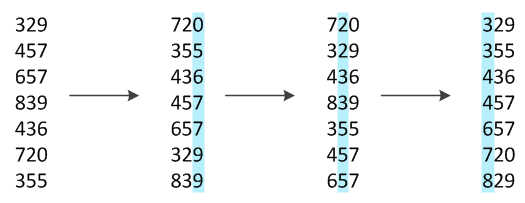
\includegraphics[width=325px,height=140px]{sort2.png}
	
\end{frame}

%%%%%%%%%%%%%%%%%%%%%%%%%%%%%%%%%%%%%%%%%%%%%%%%%%%%%%%%%%%%%%%

\begin{lstlisting}[label=some-code,caption={Реализация на Python}]


length = len(str(max(A)))
lente = len(A)
for i in range(length):
  B = [[] for k in range(lente)]
    for j in range(len(A)):
       n = A[i] // 10**i % 10
       B[n].append(A[i])
    A = []
   for k in range(lente):
       A = A + B[k]


\end{lstlisting}

%%%%%%%%%%%%%%%%%%%%%%%%%%%%%%%%%%%%%%%%%%%%%%%%%%%%%%%%%%%%%%%

\begin{frame}[t]
	\frametitle{Insertion Sort}
	\begin{itemize}
		\pause 
		\item На каждом шаге алгоритма мы выбираем один из элементов входных данных и вставляем его на нужную позицию в уже отсортированной части массива, до тех пор пока весь набор входных данных не будет отсортирован. Метод выбора очередного элемента из исходного массива произволен, однако обычно (и с целью получения устойчивого алгоритма сортировки), элементы вставляются по порядку их появления во входном массиве. \pause
	   \href{images/gif3.gif}{Insertion sort}
	\end{itemize}
\end{frame}
%%%%%%%%%%%%%%%%%%%%%%%%%%%%%%%%%%%%%%%%%%%%%%%%%%%%%%%%%%%%%%%

\begin{lstlisting}[label=some-code,caption={Реализация на Python}]

for i in range(len(data)):
    j = i - 1 
    key = data[i]
    while (data[j] > key and j >= 0):
      data[j + 1] = data[j]
      j -= 1
    data[j + 1] = key

\end{lstlisting}

%%%%%%%%%%%%%%%%%%%%%%%%%%%%%%%%%%%%%%%%%%%%%%%%%%%%%%%%%%%%%%%

\begin{frame}[t]
	\frametitle{Bucket Sort}
	\begin{itemize}
		\pause
		\item Для карманной сортировки нужно разбить элементы массива входных данных на k блоков (карманов, корзин). Далее каждый из таких блоков сортируется либо другой сортировкой, либо рекурсивно тем же методом разбиения. После сортировок внутри каждых блоков данные записываются в массив в порядке разбиения на блоки. При этом нужно учитывать, что данная сортировка работает только в том случае, если разбиение на блоки производится таким образом, чтобы элементы каждого следующего блока были больше предыдущего.\pause
		\item 	Карманная сортировка сильно деградирует при большом количестве мало отличных элементов (большинство элементов попадёт в одну корзину). Поэтому такой тип сортировки использовать, когда велика вероятность того, что числа редко повторяются (например, последовательность случайных чисел) \pause
	\end{itemize}
\end{frame}


\begin{frame}[t]
	\frametitle{Bucket Sort}
		\begin{itemize}
		\item Пример сортировки вычёрпыванием
		\item \href{https://www.cs.usfca.edu/~galles/visualization/BucketSort.html}{Bucket Sort}
	\end{itemize}
		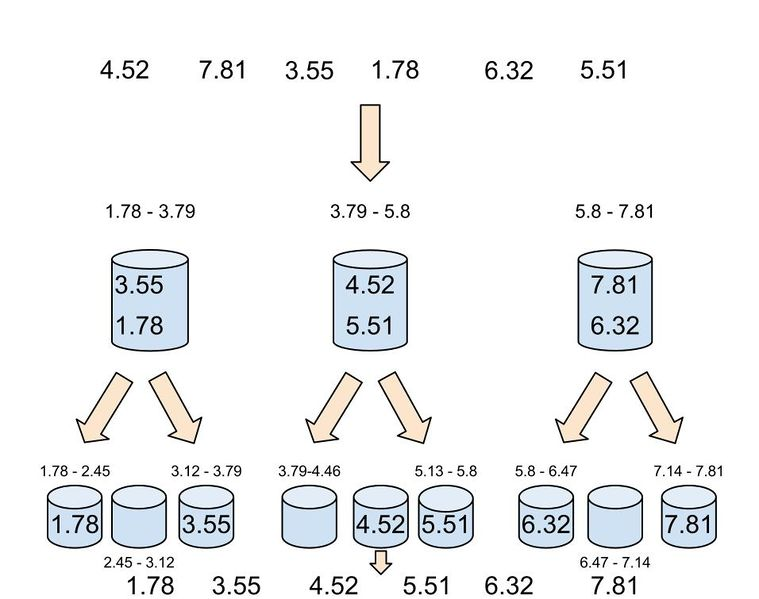
\includegraphics[width=290px,height=180px]{sort3.jpg}
	

\end{frame}



\begin{lstlisting}[label=some-code,caption={Реализация на Python}]
def bucketSort(x): 
arr = [] 
slot_num = 10 
for i in range(slot_num): 
    arr.append([]) 

for j in x: 
    index_b = int(slot_num * j)  
    arr[index_b].append(j) 

for i in range(slot_num): 
    arr[i] = insertionSort(arr[i]) 
k = 0
for i in range(slot_num): 
    for j in range(len(arr[i])): 
        x[k] = arr[i][j] 
        k += 1
return x 
\end{lstlisting}

\begin{frame}[t]
	\frametitle{Bucket Sort}%СКОРЕЕ ВСЕГО НУЖНО УБРАТЬ ВЕСЬ СЛАЙД%
	\begin{itemize}
		\item Теорема. Алгоритм SortB работает за время O(N) в среднем, где N – количество сортируемых элементов.
		
		Доказательство. Пусть p=1/N. Вероятность попадания в один контейнер k элементов равна pk=СNk pk (1-p)N-k  (биноминальное распределение).  Время работы алгоритма сортировки в одном контейнере равно S O(k2), где k – количество элементов, попавших в i-ый контейнер.
		
		Согласно свойствам биномиального распределения, среднее (математическое ожидание) количество элементов в контейнере равно M(k)= Sk  pkk=Np=1.  Средне-квадратичное отклонение от среднего значения (дисперсия) количества элементов в контейнере равно D(k)= S k  pk(k- M(k))2=S  k pk(k-1)2=Np(1-p)=1-1/N.
		
		D(k)=M(k2) – (M(k))2  из чего сразу следует M(k2)=D(k) +(M(k))2=2-1/N. Итого, среднее время сортировки одного контейнера равно O(1), а среднее время сортировок N контейнеров равно O(N).
	\end{itemize}
\end{frame}


\begin{frame}[t]
	\frametitle{Pancake Sort}
	\begin{itemize}
		\item Алгоритм сортировки с помощью одной операции — переворота элементов последовательности до какого-то индекса (префикса последовательности). Разумеется, разрешены сравнения, при оценке времени работы этого алгоритма оценивается количество переворотов, а не сравнений. Название алгоритма пошло от изначальной задачи отсортировать стопку блинов по возрастанию размера.
		\item \href{images/gif4.gif}{Pancake sort}
				\begin{rstate}
			Алгоритм корректен и работает за линейное время.    
		\end{rstate}
	\end{itemize}
\end{frame}

\begin{frame}[t]
	\frametitle{Pancake Sort}
	\begin{itemize}
		\item Покажем, что любую последовательность можно отсортировать с помощью блинной сортировки. Для этого будет предложен алгоритм, позволяющий отсортировать любой массив, сделав не более 2n операций, где n — размер массива. Найдём max элемент последовательности с номером i и развернём префикс массива до i-го элемента. Теперь max элемент находится в начале массива. Развернём весь массив, теперь max элемент находится в конце массива. Сделаем то же самое рекуррентно для префикса длины n—1. Переместим второй по возрастанию элемент в конец подотрезка, после чего последние два элемента будут отсортированы, и продолжим для префикса длины n—2. Таким образом, на каждой итерации мы сделаем две операции, и всего итераций будет не больше n. Тогда суммарное количество операций не превосходит 2n и любая последовательность может быть отсортирована таким образом.
		
	\end{itemize}
\end{frame}


\begin{lstlisting}[label=some-code,caption={Реализация на Python}]


def pancake(data):

 if len(data) > 1:
   for i in range(len(data), 1, -1):
   mxin=data.index(max(data[:i]))
   if(mxin==(i-1)):
      continue
   data[:(mxin+1)]=list(reversed(data[:(mxin+1)]))
   data[:i]=list(reversed(data[:i]))

return data

\end{lstlisting}

\begin{frame}[t]
	\frametitle{Литература}
	\begin{itemize}
\item wikipedia.org
\item Алгоритмы и алгоритмические языки-Староверов, В.М.,МГУ им. М.В.Ломоносова,2018.
\item neerc.ifmo.ru	
\item Алгоритмы: построение и анализ-Книга, Клиффорд Штайн, Рональд Линн Ривест, Томас Кормен, и Чарльз Эрик Лейзерсон.
\item habr.com		
	\end{itemize}
\end{frame}


\end{document}